\Opensolutionfile{ans}[ans/ans0D6-OT2]
\setcounter{ex}{0}
\subsubsection{Đề số 2}

\begin{ex}%[0D2Y2]
	Đường thẳng $y = 3x - 2$ không đi qua điểm nào sau đây?
	\choice
	{$Q(1;1)$}
	{\True $N(-2;-4)$}
	{$P(0;-2)$}
	{$M(-1;-5)$}
	\loigiai{
		Thay $x =  - 2;y =  - 4$ vào PTĐT thì không thỏa mãn.
	}
\end{ex}


\begin{ex}%[0D2B1]
		Trong các hàm số sau, hàm số nào đồng biến trên $\Bbb{R}$?
		\choice
		{$y=-22x+10$}
		{\True $y=22x+10$}
		{$y=-10x-22$}
		{$y=22-10x$}
		\loigiai{
			Hàm số $y=22x+10$ có $a=22>0\Rightarrow $ hàm số đồng biến trên $\Bbb{R}.$
		}
\end{ex}
	
\begin{ex}%[0D2Y1]
		Tìm tập xác định của hàm số $y=\dfrac{1}{\sqrt{x-5}}$.
		\choice
		{$(-\infty ;5]$}
		{$[5;+\infty )$ }
		{$(-\infty ;5)$}
		{\True $(5;+\infty )$}
		\loigiai{
			\begin{itemize}
				\item [$\bullet$] Hàm số xác định khi và chỉ khi $ x-5 > 0 \Leftrightarrow x > 5.$
				\item [$\bullet$] Vậy tập xác định $ \mathscr D = (5;+\infty) $.
			\end{itemize}
			}
\end{ex}

\begin{ex}%[0D2B1]
		Tập xác định của hàm số $y = \dfrac{5 + x}{\sqrt{x} - 2}$ là
		\choice
		{$\mathcal{D} = \mathbb{R}$}
		{\True $\mathcal{D} = \left[0; + \infty \right) \backslash \{ 4 \}$}
		{$\mathcal{D} = \left[0; + \infty \right) \backslash  \{ 2 \}$}
		{$\mathcal{D} = \left(0; +\infty \right)$}
		\loigiai{
		\begin{itemize}
			\item [$\bullet$] Điều kiện xác định $\heva{& x \ge 0\\& \sqrt{x}-2 \ne 0} \Leftrightarrow \heva{& x \ge 0\\& x \ne 4} $. 
			\item [$\bullet$] Suy ra tập xác định là $\mathcal{D} = \left[0; + \infty \right) \backslash \{ 4 \}$.
	\end{itemize}}
\end{ex}
	
	
\begin{ex}%[0D2B1]
	Tập xác định của hàm số $y=\sqrt{x+2}+4\sqrt{3-x}$ là
	\choice
	{$\mathscr{D}=[3; +\infty)$}
	{\True $[-2; 3]$}
	{$(-\infty; 3]$}
	{$(-2; 3)$}
	\loigiai{ 
		\begin{itemize}
		\item [$\bullet$] Hàm số xác định $\Leftrightarrow \heva{ & x+2\ge 0 \\  & 3-x\ge 0} \Leftrightarrow \heva{& x\ge -2 \\  & x\le 3} \Leftrightarrow -2\le x\le 3$.
		\item [$\bullet$] Vậy tập xác định của hàm số là $\mathscr{D}=\left[-2; 3\right]$. 
		\end{itemize}
		}
\end{ex}
	
\begin{ex}%[0D2B1]
	Cho hàm số $y=f(x)=\heva{&x^2+4x &\text{khi} \quad & x\le -1\\ &2x-1& \text{khi} \quad & -1<x \le 3 \\ & -x+6& \text{khi} \quad& x>3}.$\\
	Tính giá trị biểu thức $A=f(-2)+f(-1)+f(1)+f(2) + f(3) +f(4)$
	\choice
	{\True $A=4$}
	{$A=63$}
	{$A=2$}
	{$A=8$}
	\loigiai{}
\end{ex}
	
\begin{ex}%[0D2Y1]
	Tập xác định của hàm số $y=\dfrac{x^2+\sqrt{3-x}}{x-2}$ là
	\choice
	{$(-\infty;3)\backslash \{2\}$}
	{$(2;3]$}
	{\True $(-\infty;3]\backslash \{2\}$}
	{$(-\infty;3]$}
	\loigiai{
	\begin{itemize}
	\item [$\bullet$] Điều kiện xác định $\heva{&3-x \ge 0\\& x-2 \ne 0} \Leftrightarrow \heva{&x \le 3\\& x \ne 2}$.
	\item [$\bullet$] Suy ra tập xác định là $(-\infty;3]\backslash \{2\}$.
	\end{itemize}}
\end{ex}
	
\begin{ex}%[0D2B1]
	Hàm số nào dưới đây có tập xác định là $\mathbb{R}$?
	\choice
	{$y=\dfrac{3x}{x^2-4}$}
	{$y=x^2-2\sqrt{x-1}-3$}
	{\True $y=x^2-\sqrt{x^2+1}-3$}
	{$y=\dfrac{2\sqrt{x}}{x^2+4}$}
	\loigiai{
	Xét các phương án
	\begin{itemize}
		\item [$\bullet$] $y=\dfrac{3x}{x^2-4}$ xác định $\Leftrightarrow x^2-4 \ne 0 \Leftrightarrow x\ne \pm 2$.
		\item [$\bullet$] $y=x^2-2\sqrt{x-1}-3$ xác định $\Leftrightarrow x-1>0 \Leftrightarrow x>1$.
		\item [$\bullet$] $y=\dfrac{2\sqrt{x}}{x^2+4}$ xác định $\Leftrightarrow x>0$.
	\end{itemize}
		}
\end{ex}
	
\begin{ex} 
	\immini{Cho hàm số $y=f(x)$ có đồ thị trên miền $[-3;5]$ như sau. Hàm số nghịch biến trên khoảng nào sau đây?
	\choice
	{$(-3;0)$}
	{\True $(0;1)$}
	{$(0;3)$ }
	{$(1;3)$ }}{
	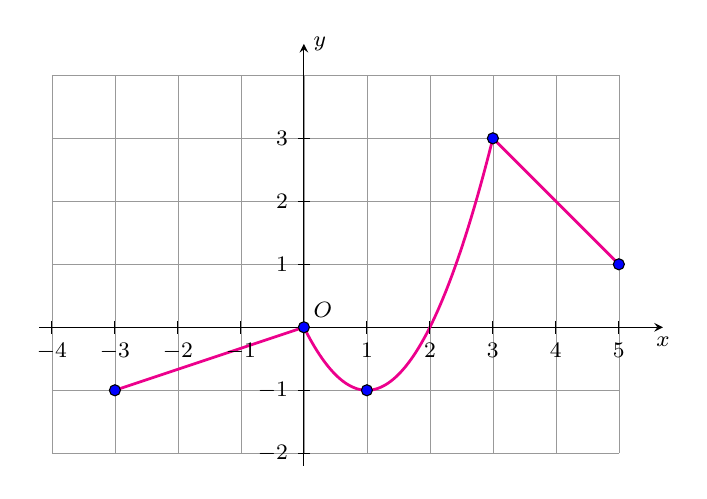
\begin{tikzpicture}[smooth,samples=300,scale=0.8,>=stealth,font=\footnotesize]
		\draw[line width=0.1pt,gray!80] (-4,-2) grid (5,4);
		\draw[->] (-4.2,0)--(5.7,0) node[below]{$x$};
		\draw[->] (0,-2.2)--(0,4.5) node[right]{$y$};
		\draw (0,0) node[above right]{$O$};
		\draw[line width=1pt,domain=0:3,magenta] plot(\x,{(\x-1)^2-1});
		\draw[line width=1pt,magenta] (-3,-1)--(0,0) (3,3)--(5,1);
		\draw[fill=blue] (-3,-1) circle(2.5pt) (0,0) circle(2.5pt) (3,3) circle(2.5pt) (5,1) circle(2.5pt) (1,-1) circle(2.5pt);
		\foreach \x in {-4,-3,-2,-1,1,2,3,4,5}\draw (\x,0.1)--(\x,-0.1) node [below] {\footnotesize $\x$};
		\foreach \y in {-2,-1,1,2,3}\draw (0.1,\y)--(-0.1,\y) node [left] {\footnotesize $\y$};
\end{tikzpicture}}
\end{ex}
\begin{ex}%[0D2B2]
	Tìm $m$ để hàm số $y=(-2m+1)x+m-3$ đồng biến trên $\mathbb{R}$.
	\choice        
	{\True $m<\dfrac{1}{2}$}
	{$m>\dfrac{1}{2}$}
	{$m<3$}
	{$m>3$}
	\loigiai{
		Hàm số 	$y=(-2m+1)x+m-3$ đồng biến trên $\mathbb{R}$ khi $-2m+1>0\Leftrightarrow m<\dfrac{1}{2}$.
		}
\end{ex}
	
\begin{ex}%[0D2Y3-2]
	Hàm số nào trong các hàm sau đây \textbf{không} phải là hàm số bậc hai?
	\choice
	{$y=f(x)=\sqrt{3}x^2+x-4$}
	{\True $y=f(x)=x^2+\dfrac{1}{x}-5$}
	{$y=f(x)=-2x(x-1)$}
	{$y=f(x)=2(x^2+1)+3x-1$}
	\loigiai{
		Ham số $y=f(x)=x^2+\dfrac{1}{x}-5$ không phải là hàm số bậc hai.
	}
\end{ex}


\begin{ex}%[0D2B3]
	Tìm toạ độ đỉnh $I$ của parabol $y=x^2+4x+5$.
	\choice
	{$I(0;5)$}
	{$I(1;10)$}
	{$I(-1;2)$}
	{\True $I(-2;1)$}
	\loigiai{
	\begin{itemize}
		\item [$\bullet$] Hoành độ đỉnh $x=-\dfrac{b}{2a}=-2$.
		\item [$\bullet$] Với $x=-2$, thay vào hàm ta tính được $y=1$. 
	\end{itemize}
	Vậy tọa độ đỉnh là $I(-2;1)$.
	}
\end{ex}

\begin{ex}%[0D2K3]
	\immini{Hình vẽ bên là đồ thị của hàm số nào sau đây?
	\motcot
	{$y=x^2+4x+5$}
	{$y=x^2+2x-1$}
	{\True $y=2x^2+8x+5$}
	{$y=x^2+4x-3$}
	}{
	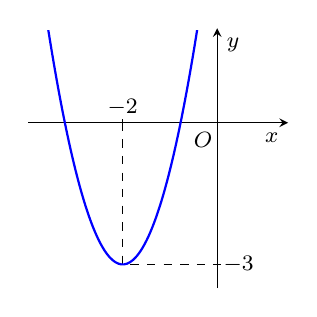
\begin{tikzpicture}[scale=0.6,>=stealth,x=1cm,y=1cm]
			\draw (-0.3,0) node[below] {\footnotesize $O$};
			\draw[->] (-4,0) -- (1.5,0) node [below left] {\footnotesize$x$};
			\draw[->] (0,-3.5) -- (0,2) node [below right] {\footnotesize$y$};
			\foreach \x/\xtext in {-2/-2}
			\draw[shift={(\x,0)}] (0pt,2pt)--(0pt,-2pt) node[above] {\footnotesize $\xtext$};
			\foreach \y/\ytext in {-3/-3}
			\draw[shift={(0,\y)}] (2pt,0pt)--(-2pt,0pt) node[right] {\footnotesize $\ytext$};
			\draw[dashed,thin] (-2,0)--(-2,-3)--(0,-3);
			\clip (-3.95,-3.45) rectangle (0.95,1.95);
			\draw[thick, color=blue,smooth,samples=100,domain=-5:1] plot(\x,{2*(\x)^2+8*(\x)+5});
			\end{tikzpicture}
		}
	\loigiai{
		Đồ thị hàm số cắt trục tung tại điểm có tung độ dương nên loại phương án B và D.\\
		Đồ thị qua điểm $(-2;-3)$ nên phương án $y=2x^2+8x+5$ thỏa mãn.
	}
\end{ex}
	
\begin{ex}%[0D2B3-3]%
	\immini{Đường cong ở hình bên là đồ thị của một trong bốn hàm số dưới đây. Hàm số đó là hàm số nào?
	\choice
	{\True $y=-x^2+4x$}
	{$y=-x^2+3x$}
	{$y=-2x^2+2x+1$}
	{$y=x^2-3x+2$}
	}{	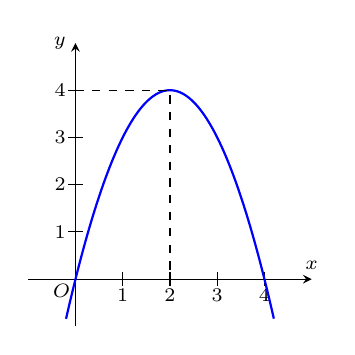
\begin{tikzpicture}[x=0.5cm,y=0.5cm,>=stealth,scale=1.2]
				\draw[->] (-1,0) -- (5,0) node[above]{\scriptsize $x$};
				\draw[->] (0,-1) -- (0,5) node[left]{\scriptsize $y$};
				\draw (0.1,0.1) node[below left]{\scriptsize $O$};
				\foreach \i in {1,2,3,4}{
					\draw (\i,0) node[below]{\scriptsize $\i$};
					\draw (0,\i) node[left]{\scriptsize $\i$};
					\draw (0.15,\i) -- (-0.15,\i) (\i,0.15) -- (\i,-0.15);
				}
				\draw[samples=100,domain=-0.2:4.2,thick,blue] plot (\x,{-(\x)^2+4*(\x)});
				\draw[dashed] (0,4) -- (2,4) -- (2,0);
			\end{tikzpicture}
		}
	\loigiai{
	Đồ thị là một parabol nên hàm số có dạng $y=ax^2+bx+c$. Ta thấy đồ thị đi qua các điểm $(0;0), (2;4)$ và $(4;0)$ nên ta có
	$$\heva{& c=0\\ & 4a+2b+c=4\\ & 16a+4b+c=0}\Leftrightarrow \heva{& a=-1\\ & b=4\\ &c=0.}$$
	Vậy hàm số cần tìm là $y=-x^2+4x$.
	}
\end{ex}

\begin{ex}%[0D2B3-3]%
	\immini{Cho hàm số $y=ax^2+bx+c$ có đồ thị như hình vẽ bên. Mệnh nào sau đây đúng?
		\choice
		{\True $a>0$, $b>0$, $c>0$}
		{$a>0$, $b<0$, $c>0$}
		{$a<0$, $b>0$, $c>0$}
		{$a>0$, $b=0$, $c>0$}
}{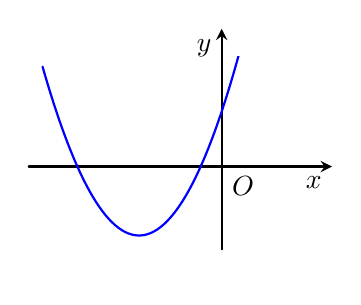
\begin{tikzpicture}[line join=round, line cap=round,>=stealth,thick,scale=0.7]
			\tikzset{label style/.style={font=\footnotesize}}
			\draw[->] (-3.5,0)--(2,0) node[below left] {$x$};
			\draw[->] (0,-1.5)--(0,2.5) node[below left] {$y$};
			\draw (0,0) node [below right] {$O$};
			\begin{scope}
				\clip (-3.5,-2) rectangle (2,2);
				\draw[samples=200,domain=-3.25:2,smooth,variable=\x,blue] plot (\x,{1*(\x)^2+3*(\x)+1});
			\end{scope}
\end{tikzpicture}}
	\loigiai{
		Đồ thị có bề lõm quay lên trên $ \Rightarrow a>0$.\\
		Trục đối xứng $x=-\dfrac{b}{2a}<0 \Rightarrow a.b>0 \Rightarrow b>0$.}
\end{ex}

\begin{ex}%[0D2B3-1]
	Tập giá trị của hàm số $y=f(x)=-2x^2+\sqrt{2}x+1$ là
	\choice
	{$T=\left(-\dfrac{5}{4};+\infty \right)$}
	{$T=\left[-\dfrac{5}{4};+\infty \right)$}
	{$T=\left(-\infty;\dfrac{5}{4}\right)$}
	{\True $T=\left(-\infty;\dfrac{5}{4}\right]$}
	\loigiai{
		Ta có tọa độ đỉnh $I\left(\dfrac{\sqrt{2}}{4};\dfrac{5}{4}\right)   $.\\
		Có $ a=-2<0 $ nên parabol có bề lõm quay xuống dưới.\\
		Do đó tập giá trị của hàm số đã cho là $T= \left (-\infty;\dfrac{5}{4}\right ] $.	
	}
\end{ex}

\begin{ex}%[0D2K3-3]%
	\immini{Cho hàm số bậc hai có đồ thị như hình bên. Tập xác định và tập giá trị của hàm số theo thứ tự là
		\choice
		{$[-1; 7]$ và $(-\infty; 8]$}
		{$(-\infty; +\infty)$ và $[8; +\infty)$}
		{\True $(-\infty; +\infty)$ và $(-\infty; 8]$}
		{$[-1; 9]$ và $[-2; 9]$}
	}{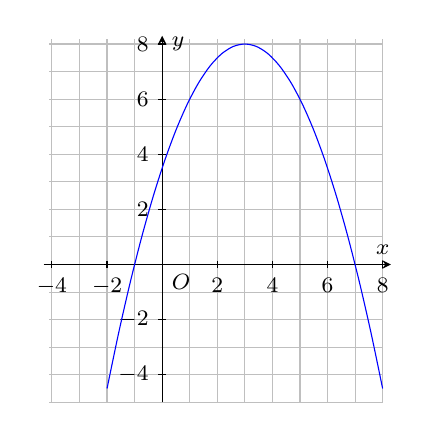
\begin{tikzpicture}[x=0.5cm,y=0.5cm,scale=.7,>=stealth]
			\draw[color=gray!50] (-4.1,-5) grid[step=5mm] (8,8.2);
			\foreach \x in {-4,-2,2,4,6,8}
			\draw[shift={(\x,0)},color=black] (0pt,2pt) -- (0pt,-2pt) node[below] {\footnotesize $\x$};
			\draw[->] (0,-5) -- (0,8.3);
			\foreach \y in {-4,-2,2,4,6,8}
			\draw[shift={(0,\y)},color=black] (2pt,0pt) -- (-2pt,0pt) node[left] {\footnotesize $\y$};
			\draw[->] (-4.3,0) -- (8.3,0);
			\draw[-,smooth,domain=-2:8,blue] plot(\x,{-.5*(\x)^2+3*(\x)+3.5});
			\draw(0,0)node[below right]{\footnotesize$O$};
			\draw(8,0)node[above]{\footnotesize$x$};
			\draw(0,8)node[right]{\footnotesize$y$};
	\end{tikzpicture}}
	\loigiai{
		Đồ thị có dạng đồ thị hàm số bậc hai nên tập xác định là $(-\infty; +\infty)$. Điểm cao nhất của đồ thị là $(3; 8)$ nên tập giá trị là $(-\infty; 8]$.}
\end{ex}

\begin{ex}%[0D2B3]
	Giá trị nhỏ nhất của biểu thức $f(x)=x^2-4x+1$ là 
	\choice
	{$3$}
	{$2$}
	{$-2$}
	{\True $-3$}
	\loigiai{
	\begin{itemize}
		\item [$\bullet$] Cách 1: Lập bảng biến thiên của hàm số.
		\item [$\bullet$] Cách 2: Phân tích $f(x)=x^2-4x+1=(x-2)^2-3 \ge -3, \forall x \in \mathbb{R}$. \\
		Suy ra $f_{\min}=-3$ khi $x=2$.
	\end{itemize}
	}
\end{ex}
	
\begin{ex}%[0D2Y3]
	Đồ thị hàm số $y=2x^2 - x - 3$ có trục đối xứng là 
	\choice
	{\True $x=\dfrac{1}{4}$}
	{$x= - \dfrac{1}{2}$}
	{$x= - \dfrac{1}{4}$}
	{$x=\dfrac{1}{2}$}
	\loigiai{
		Phương trình trục đối xứng $x=-\dfrac{b}{2a}=\dfrac{1}{4}$.}
\end{ex}

\begin{ex}%[0D2B3]
	Cho hàm số $y =  - x^2 + 4x + 3$. Chọn khẳng định đúng.
	\choice
	{Hàm số đồng biến trên $\mathbb{R}$}
	{Hàm số đồng biến trên $(2, + \infty )$}
	{\True Hàm số nghịch biến trên $(2, + \infty )$}
	{Hàm số nghịch biến trên $\mathbb{R}$}
	\loigiai{
		Tọa độ đỉnh $(2;7)$.\\
		Bảng biến thiên:
		\begin{center}
				
\begin{tikzpicture}
				\tkzTabInit[nocadre=false, lgt=1,espcl=3]  
				{$x$/0.7, $y$/2}  
				{$-\infty$, $2$, $+\infty$}  
				\tkzTabVar{-/ $-\infty$, +/ $7$ , -/ $-\infty$}  
				\end{tikzpicture}
			\end{center}
		Dựa vào bảng biến thiên, ta có hàm số đồng biến trên $(- \infty ,2)$ và hàm số nghịch biến trên $(2, + \infty )$.
		}
\end{ex}
	
\begin{ex}%[0D2K3]
	Biết rằng đồ thị hàm số $y = mx + n$ đi qua đỉnh của parabol $y = x^2 - 2x + 3$. Hãy tính $m + n$.
	\choice
	{$0$}
	{$1$}
	{\True $2$}
	{$-2$}
	\loigiai
	{
	Đỉnh của parabol $y = x^2 - 2x + 3$ là $I(1;2)$.\\
		Vì đường thẳng $y = mx + n$ đi qua đỉnh $I(1;2)$ nên $m + n = 2$.
		}
\end{ex}
	
\begin{ex}%[0D2B3]
\immini{Hàm số nào sau đây có bảng biến thiên như hình vẽ dưới? 
	\choice
	{ $y = -x^2 -4x -9$}
	{ $y = x^2 + 4x - 5$}
	{\True $y = x^2 + 4x - 1$}
	{ $y = x^2 + 2x -5$}}{
	
\begin{tikzpicture}
		\tkzTabInit[nocadre=false, lgt=1, espcl=2]{$x$ /0.6,$y$ /1.5}{$-\infty$,$-2$,$+\infty$}
		%\tkzTabLine{,+,0,-, d ,-,0,+,}
		\tkzTabVar{+/$+\infty$ , -/ $-5$ /, +/$+\infty$ /}
		\end{tikzpicture}}
	\loigiai{
		Bảng biến thiên của hình bên tương ứng với $a>0$, ta loại phương án A.\\
		Tọa độ đỉnh $(-2;-5)$ nên chỉ có phương án $y = x^2 + 4x - 1$ thỏa mãn.
		}   
\end{ex}
	
\begin{ex}%[0D2G3]
	Xác định $(P): y=ax^2+bx+c$ biết hàm số đạt giá trị nhỏ nhất bằng $\dfrac{3}{4}$ khi $x=\dfrac{1}{2}$ và nhận giá trị bằng $1$ khi $x=1$.
	\choice
	{$y=x^2+x-1$}
	{\True $y=x^2-x+1$}
	{$y=2x^2-x+1$}
	{$y=x^2-x$}
	\loigiai{
		Hàm số đạt giá trị nhỏ nhất bằng $\dfrac{3}{4}$ khi $x=\dfrac{1}{2}$ nên
		$$
		\heva{
			& a>0   \\
			& -\dfrac{b}{2a}=\dfrac{1}{2} \\
			& a\left( \dfrac{1}{2}\right)^2+b\dfrac{1}{2}+c=\dfrac{3}{4}}
		\Leftrightarrow
		\heva{
			& a>0 &&  \\
			& b=-a &(1)&\\
			& a+2b+4c=3 &(2)&}
		$$
		Hàm số nhận giá trị bằng $1$ khi $x=1$ nên $a+b+c=1 \,(3)$\\
		Từ (1),(2) và (3) tìm được $a=1; b=-1; c=1$. Vậy  $y=x^2-x+1$.
		
	}
\end{ex}
	
\begin{ex}%[0D2G3-3]%
	\immini{Cho hai hàm số $y=a_1 x^2+b_1 x +c_1$ và $y=a_2 x^2+b_2 x + c_2$ với $a_1$, $a_2$, $b_1$, $b_2$, $c_1$, $c_2$ là các số thực, lần lượt có đồ thị là $(C_1)$ và $(C_2)$ như hình bên. Mệnh đề nào dưới đây đúng?
		\choice
		{$a_1>a_2, b_1>b_2, c_1>c_2$}
		{$a_1<a_2, b_1<b_2, c_1<c_2$}
		{$a_1>a_2, b_1<b_2, c_1>c_2$}
		{\True $a_1<a_2, b_1>b_2, c_1<c_2$}
	}
	{
		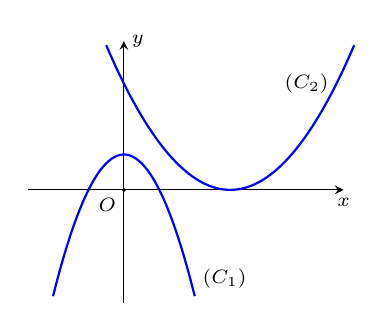
\begin{tikzpicture}[>=stealth, x=1cm, y=1cm, scale=0.45]
			\begin{scriptsize}
				\def\xmin{-2.5} \def\xmax{6} \def\ymin{-3} \def\ymax{4};
				\draw [->] (\xmin-.2, 0)--(\xmax+.2, 0) node[below]{$x$};
				\draw [->] (0, \ymin-.2)--(0, \ymax+.2) node[right]{$y$};
				\draw [fill=black] circle (1pt) node [below left]{$O$};
				\draw (2,-2.5) node [right]{$(C_1)$} (6,3) node [left]{$(C_2)$};
				\draw[smooth,domain=-2:2,blue,thick] plot(\x,{(-1)*(\x)^(2)+1});
				\draw[smooth,domain=-0.5:6.5,blue,thick] plot(\x,{(1/3)*(\x)^(2)-2*(\x)+3});
			\end{scriptsize}
		\end{tikzpicture}
	}
	\loigiai{
		Từ hai đồ thị ta có $a_1<0,b_1=0,a_2>0,b_2<0$ và $c_1<c_2$.
		Do đó ta chọn kết quả $a_1<a_2, b_1>b_2, c_1<c_2$.}
\end{ex}

\begin{ex}%[Dự án TeX  hóa tài liệu BTN 10]%[Soạn Thầy Võ Tấn Đạt, phản biện thầy Lê Hoàng Lâm]%[0D4B5-2]%
	Cho tam thức bậc hai $f(x)=-x^2-4x+5$. Tìm tất cả giá trị của $x$ để $f(x)\geqslant 0$.
	\choice
	{$x\in (-\infty;-1]\cup [5;+\infty)$}
	{$x\in [-1;5]$}
	{\True $x\in [-5;1]$}
	{$x\in (-5;1)$}
	\loigiai{
		Ta có $f(x)=0$ $ \Leftrightarrow $ $-x^2-4x+5=0$ $ \Leftrightarrow $ $x=1$, $x=-5$.\\
		Mà hệ số $a=-1<0$ nên: $f(x)\geqslant 0$ $ \Leftrightarrow $ $x\in [-5;1]$.}
\end{ex}



\begin{ex}%[Dự án TeX  hóa tài liệu BTN 10]%[Soạn Thầy Võ Tấn Đạt, phản biện thầy Lê Hoàng Lâm]%[0D4B5-2]%
	Tìm tập nghiệm $S$ của bất phương trình $x^2-4x+4>0$.
	\choice
	{\True $S=\mathbb{R}\setminus \{2\}$}
	{$S=\mathbb{R}$}
	{$S=(2;+\infty)$}
	{$S=\mathbb{R}\setminus \{-2\}$}
	\loigiai{
		Bảng xét dấu:
		\begin{center}
			
\begin{tikzpicture}
				\tkzTabInit[nocadre=false,lgt=2.5,espcl=2.4]
				{$x$ /0.7,$x^2-4x+4$ /0.7}
				{$-\infty$,$2$,$+\infty$}
				\tkzTabLine{,+,$0$,+}
			\end{tikzpicture}
		\end{center}
		Tập nghiệm của bất phương trình là $S=\mathbb{R}\setminus \{2\}$.}
\end{ex}

\begin{ex}%[0D4K5-2]
	Tam thức $f(x)=x^2-(m+2)x+8m+1$ \textbf{không} âm với mọi $x \in \mathbb{R}$ khi và chỉ khi
	\choice
	{$m>28$}
	{\True $0\le m\le 28$}
	{$m<1$}
	{$0<m<28$}
	\loigiai
	{
		Tam thức $f(x)$ có $a=1>0$. Do đó
		\allowdisplaybreaks
		\begin{eqnarray*}
			f(x) \geq 0,\forall x \Leftrightarrow (m+2)^2-4(8m+1) \leq 0 \Leftrightarrow m^2-28m\leq 0 \Leftrightarrow 0\leq m\leq 28.
		\end{eqnarray*}
		Vậy $0\le m\le 28$ là các giá trị cần tìm.
	}
\end{ex}

\begin{ex}
	Tập nghiệm của phương trình $\sqrt{2 x^{2}-9 x-9}=3-x$ là
	\choice
	{$S=\{6\}$}
	{$S=\varnothing$}
	{\True $S=\{-3\}$}
	{$S=\{-3 ; 6\}$}
	\loigiai{
		Bình phương hai vế ta được 
		$$2x^2-9x-9=9-6x+x^2 \Leftrightarrow x^2-3x-18=0 \Leftrightarrow x=6,\, x=-3$$
		Thử lại, ta được $x=-3$ thoả.
	}
\end{ex}

\begin{ex}
	Tập nghiệm của phương trình $\sqrt{2 x^{2}-5 x+1}=\sqrt{x^{2}+2 x-9}$ là
	\choice
	{$S=\{2\}$}
	{\True $S=\{5\}$}
	{$S=\varnothing$}
	{$S=\{2 ; 5\}$}
	\loigiai{
		Bình phương hai vế ta được 
		$$2x^2-5x+1=x^2+2x-9 \Leftrightarrow x^2-7x+10=0 \Leftrightarrow x=5,\, x=2$$
		Thử lại, ta được $x=5$ thoả.
	}
\end{ex}

\begin{ex}%[0D2G3-5]
	Giả sử một máy bay cứu trợ đang bay theo phương ngang và bắt đầu thả hàng từ độ cao $80 \mathrm{~m}$, lúc đó máy bay đang bay với vận tốc $50 \mathrm{~m} / \mathrm{s}$. Để thùng hàng cứu trợ rơi đúng vị trí được chọn, máy bay cần bắt đầu thả hàng từ vị trí nào? 
	\begin{center}
		%\foreach \i in{1}{
			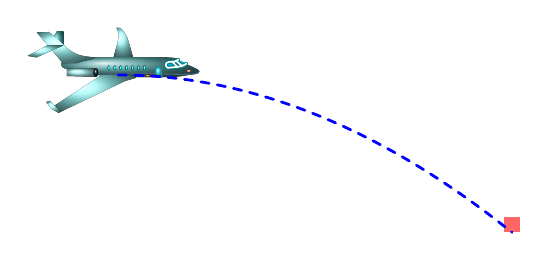
\begin{tikzpicture}[font=\footnotesize, line join=round, line cap=round, >=stealth]
				\def\i{1}
				%Cânh đuôi trái
				\tikzset{Icon-Maybay/.pic={
						\begin{scope}
							\fill[ball color =cyan!40!gray,rounded corners=0.02](-5.6,3)--++(60:0.8)--++(2:0.55)--++(-90:2)--cycle;
							%%Hai cánh
							\fill[ball color =cyan!90!gray!40!white](-0.4,1.5)..controls++(75:2)and++(-68:0.75)..(-0.15,4)--++(-5:0.35)..controls++(-50:0.95)and++(106:2)..(1.25,1.5)--cycle;
							%Thân
							\fill[ball color =cyan!30!gray](-4.85,1)..controls++(-90:0.6) and++(180:0.2)..(-4,0.5)--++(-12:3.3)--++(0:4)..controls++(0:2) and++(-172:1)..(6,0)..controls++(8:1)and++(-90:0.1)..(6.85,0.3)..controls++(90:0.2) and++(-30:1)..(5,1.3)..controls++(90:0.25) and++(0:8)..(-4,1.5)--cycle;
							\draw[cyan!40!black](6.85,0.3)coordinate(mui)..controls++(-90:0.5) and++(0:6)..(-2,0.2);
							% Cánh phải
							\fill[ball color =cyan!90!gray!40!white,rounded corners=0.02](-1.8,0)--++(-5:0.35)--++(-147:4.85)--++(-50:0.7)--++(25.5:6.5)..controls++(-155.5:0.5) and++(-170:0.15)..(1.5,-0.25)..controls++(120:0.5) and++(2:1)..(-1.8,0);
							\fill[ball color =cyan!90!gray!40!white,rounded corners=0.02](-6.1,-2.3)--++(-54:0.7)--++(-28:0.7)--++(25.5:.35)--++(-180:.2)--++(135:1.2)--cycle;
							%%Thân đuôi
							\fill[ball color =cyan!90!gray!40!white,rounded corners=0.02](-6.9,3.6)--++(2:1)..controls++(-35:2) and++(178:2.3)..(-2,1.5)..controls++(-90:0.2) and++(20:1)..(-3.5,1)--++(180:1.2)--cycle;
							%%Đuôi
							\fill[ball color =cyan!90!gray!40!white,rounded corners=0.02](-6,2.5)--++(0:1.35)--++(-156:2.5)--++(170:0.75)--cycle;
							\fill[ball color =cyan!70!gray!40!white,rounded corners=0.02](-1.9,-0.17)--++(90:0.72)--++(181:2.45)--++(-90:0.6)--cycle;
							\fill[ball color =cyan!90!gray!10!black,line width=0.02,draw=cyan!30!black,rounded corners=0.005](-1.9,-0.18)arc(-90:270:0.2 and 0.38);
							%%Cửa kính
							\fill[cyan](5.05,1.3)--++(-25:0.8)..controls++(-140:0.55)and++(10:0.5)..(4.2,0.6)..controls++(180:0.15) and++(182:0.45)..(4.3,1.1)..controls++(2:0.5) and++(-135:0.2)..(5.1,1.3);
							\draw[draw=teal,double,distance=0.03](5.05,1.3)++(-26:0.8)..controls++(-140:0.55)and++(10:0.5)..(4.2,0.6)foreach \i in{1,2,...,4}{coordinate[pos=\i/4](B\i)}..controls++(180:0.15) and++(182:0.45)..(4.3,1.1)..controls++(2:0.5) and++(-135:0.2)..(5.1,1.3)foreach \i in{1,2,...,10}{coordinate[pos=\i/10](A\i)}(A2)--(B2)(A6)--(B1);
							%Ô cửa trên thân máy bay
							\foreach \i in {0,1,...,6}
							\fill[ball color=cyan](-0.8+0.5*\i,0.4)arc(-90:270:0.1 and 0.2);
							\fill[draw=cyan!10!teal,ball color=cyan!80!gray,rounded corners=0.015](3.2,-0.2)--++(95:0.9)--++(0:0.5)--++(-85:0.9)--cycle;
							\pgfmathsetmacro{\j}{int(mod(\i,2))}
							\ifnum \j=1
							\begin{scope}[opacity=1]
								\fill[ball color=orange](2.5,-0.15)arc(-90:270:0.2 and 0.1);
								\fill[ball color=orange!50!red!50!white,rotate around={10:(6,0.25)}](6,0.25)arc(-90:270:0.2 and 0.1);
							\end{scope}
							\else
							\begin{scope}[opacity=0.4]
								\fill[ball color=orange](2.5,-0.15)arc(-90:270:0.2 and 0.1);
								\fill[ball color=orange!50!red!50!white,rotate around={10:(6,0.25)}](6,0.25)arc(-90:270:0.2 and 0.1);
							\end{scope}
							\fi
						\end{scope}
				}}
				\path(0,2)pic[scale=0.15]{Icon-Maybay};
				%	\draw[->] (0,0)--(0,3)node[left]{$y$};
				%	\draw[->] (0,0)--(6,0)node[above]{$x$};
				%	\draw[fill=black] (0,0)node[below left]{$O$} circle(1pt);
				\fill[red!60] (4.9,0)--(5.1,0)--(5.1,0.2)--(4.9,0.2)--cycle;
				\draw[dashed,color=blue,line width=1pt,samples=150,smooth,domain=0:5] plot(\x,{-0.08*(\x)^2+2});
				%	\draw (3,1.7)node[right]{$\heva{x&=50t\\y&=80-5t^2}$};
				
			\end{tikzpicture}
			%}
	\end{center}
	\textit{Biết rằng nếu chọn gốc toạ độ là hình chiếu trên mặt đất của vị trí hàng cứu trợ bắt đầu được thả, thì tọa độ của hàng cứu trợ được cho bởi hệ sau:
	\[\heva{x&=v_0t\\ y&=h-\dfrac{1}{2}gt^2.}\]
	Trong đó, $v_{0}$ là vận tốc ban đầu và $h$ là độ cao tính từ khi hàng rời máy bay và chuyển động này được xem là chuyển động ném ngang.}
\choice
{320 m}
{180 m}
{\True 200 m}
{230 m}
	\loigiai{
		\begin{center}
			%\foreach \i in{1}{
				\begin{tikzpicture}[font=\footnotesize, line join=round, line cap=round, >=stealth]
					\def\i{1}
					%Cânh đuôi trái
					\tikzset{Icon-Maybay/.pic={
							\begin{scope}
								\fill[ball color =cyan!40!gray,rounded corners=0.02](-5.6,3)--++(60:0.8)--++(2:0.55)--++(-90:2)--cycle;
								%%Hai cánh
								\fill[ball color =cyan!90!gray!40!white](-0.4,1.5)..controls++(75:2)and++(-68:0.75)..(-0.15,4)--++(-5:0.35)..controls++(-50:0.95)and++(106:2)..(1.25,1.5)--cycle;
								%Thân
								\fill[ball color =cyan!30!gray](-4.85,1)..controls++(-90:0.6) and++(180:0.2)..(-4,0.5)--++(-12:3.3)--++(0:4)..controls++(0:2) and++(-172:1)..(6,0)..controls++(8:1)and++(-90:0.1)..(6.85,0.3)..controls++(90:0.2) and++(-30:1)..(5,1.3)..controls++(90:0.25) and++(0:8)..(-4,1.5)--cycle;
								\draw[cyan!40!black](6.85,0.3)coordinate(mui)..controls++(-90:0.5) and++(0:6)..(-2,0.2);
								% Cánh phải
								\fill[ball color =cyan!90!gray!40!white,rounded corners=0.02](-1.8,0)--++(-5:0.35)--++(-147:4.85)--++(-50:0.7)--++(25.5:6.5)..controls++(-155.5:0.5) and++(-170:0.15)..(1.5,-0.25)..controls++(120:0.5) and++(2:1)..(-1.8,0);
								\fill[ball color =cyan!90!gray!40!white,rounded corners=0.02](-6.1,-2.3)--++(-54:0.7)--++(-28:0.7)--++(25.5:.35)--++(-180:.2)--++(135:1.2)--cycle;
								%%Thân đuôi
								\fill[ball color =cyan!90!gray!40!white,rounded corners=0.02](-6.9,3.6)--++(2:1)..controls++(-35:2) and++(178:2.3)..(-2,1.5)..controls++(-90:0.2) and++(20:1)..(-3.5,1)--++(180:1.2)--cycle;
								%%Đuôi
								\fill[ball color =cyan!90!gray!40!white,rounded corners=0.02](-6,2.5)--++(0:1.35)--++(-156:2.5)--++(170:0.75)--cycle;
								\fill[ball color =cyan!70!gray!40!white,rounded corners=0.02](-1.9,-0.17)--++(90:0.72)--++(181:2.45)--++(-90:0.6)--cycle;
								\fill[ball color =cyan!90!gray!10!black,line width=0.02,draw=cyan!30!black,rounded corners=0.005](-1.9,-0.18)arc(-90:270:0.2 and 0.38);
								%%Cửa kính
								\fill[cyan](5.05,1.3)--++(-25:0.8)..controls++(-140:0.55)and++(10:0.5)..(4.2,0.6)..controls++(180:0.15) and++(182:0.45)..(4.3,1.1)..controls++(2:0.5) and++(-135:0.2)..(5.1,1.3);
								\draw[draw=teal,double,distance=0.03](5.05,1.3)++(-26:0.8)..controls++(-140:0.55)and++(10:0.5)..(4.2,0.6)foreach \i in{1,2,...,4}{coordinate[pos=\i/4](B\i)}..controls++(180:0.15) and++(182:0.45)..(4.3,1.1)..controls++(2:0.5) and++(-135:0.2)..(5.1,1.3)foreach \i in{1,2,...,10}{coordinate[pos=\i/10](A\i)}(A2)--(B2)(A6)--(B1);
								%Ô cửa trên thân máy bay
								\foreach \i in {0,1,...,6}
								\fill[ball color=cyan](-0.8+0.5*\i,0.4)arc(-90:270:0.1 and 0.2);
								\fill[draw=cyan!10!teal,ball color=cyan!80!gray,rounded corners=0.015](3.2,-0.2)--++(95:0.9)--++(0:0.5)--++(-85:0.9)--cycle;
								\pgfmathsetmacro{\j}{int(mod(\i,2))}
								\ifnum \j=1
								\begin{scope}[opacity=1]
									\fill[ball color=orange](2.5,-0.15)arc(-90:270:0.2 and 0.1);
									\fill[ball color=orange!50!red!50!white,rotate around={10:(6,0.25)}](6,0.25)arc(-90:270:0.2 and 0.1);
								\end{scope}
								\else
								\begin{scope}[opacity=0.4]
									\fill[ball color=orange](2.5,-0.15)arc(-90:270:0.2 and 0.1);
									\fill[ball color=orange!50!red!50!white,rotate around={10:(6,0.25)}](6,0.25)arc(-90:270:0.2 and 0.1);
								\end{scope}
								\fi
							\end{scope}
					}}
					\path(0,2)pic[scale=0.15]{Icon-Maybay};
					\draw[->] (0,0)--(0,3)node[left]{$y$};
					\draw[->] (0,0)--(6,0)node[above]{$x$};
					\draw[fill=black] (0,0)node[below left]{$O$} circle(1pt);
					\fill[red!60] (4.9,0)--(5.1,0)--(5.1,0.2)--(4.9,0.2)--cycle;
					\draw[dashed,color=blue,line width=1pt,samples=150,smooth,domain=0:5] plot(\x,{-0.08*(\x)^2+2});
					\draw (3,1.7)node[right]{$\heva{x&=50t\\y&=80-5t^2}$};
					
				\end{tikzpicture}
				%}
		\end{center}
		Chọn hệ trục toạ độ có gốc toạ độ là hình chiếu trên mặt đất của vị trí hàng cứu trợ bắt đầu được thả (hình vẽ). Với $h=80 \mathrm{~m}$, vận tốc đầu của hàng cứu trợ bằng vận tốc máy bay là $50 \mathrm{~m} / \mathrm{s}$, thì phương trình chuyển động của hàng cứu trợ được cho bởi hệ sau (chọn $g=10 \mathrm{~m} / \mathrm{s}^{2}$ )
		\[\heva{&x=50t\\ &y=80-\dfrac{1}{2}\cdot 10t^2} \quad\text{hay}\quad \heva{&x=50t\\ &y=80-5t^2.}\]
		Khử $t$, ta được
		$$
		y=80-5\left(\dfrac{x}{50}\right)^{2} \quad\text {hay}\quad y=-\dfrac{x^{2}}{500}+80.
		$$
		Vị trí hàng cứu trợ rơi chạm đất chính là giao điểm của quỹ đạo parabol với trục hoành, nên tọa độ hàng cứu trợ lúc đó là $\left(x_{0} ; 0\right)$ với $x_{0}$ cho bởi $-\dfrac{x_0^2}{500}+80=0$. Giải phương trình này ta được: $x_{0}=-200$ hay $x_{0}=200$.\\
		Vị trí hàng cứu trợ rơi phải có hoành độ dương (theo cách chọn hệ trục tọa độ) nên ta nhận kết quả $x_{0}=200$.\\
		Để thùng hàng cứu trợ rơi đúng vị trí được chọn, máy bay cần bắt đầu thả hàng từ vị trí có hình chiếu của máy bay trên mặt đất cách vị trí được chọn là $200 \mathrm{~m}$.
	}
\end{ex}
\centerline{---HẾT---}
\Closesolutionfile{ans}
